\RequirePackage{luatex85}
\documentclass{standalone}

\usepackage{fontspec, unicode-math}
\setsansfont[Scale=MatchLowercase]{TeX Gyre Heros}
\setmathfont{TeX Gyre Termes Math}

\usepackage{tikz}
\usepackage{pgfplots}
\pgfplotsset{compat=1.14}

\tikzset{
  every picture/.style={font={\sffamily\normalsize}, >=stealth},
  every pin edge/.style={black}}

\begin{document}

  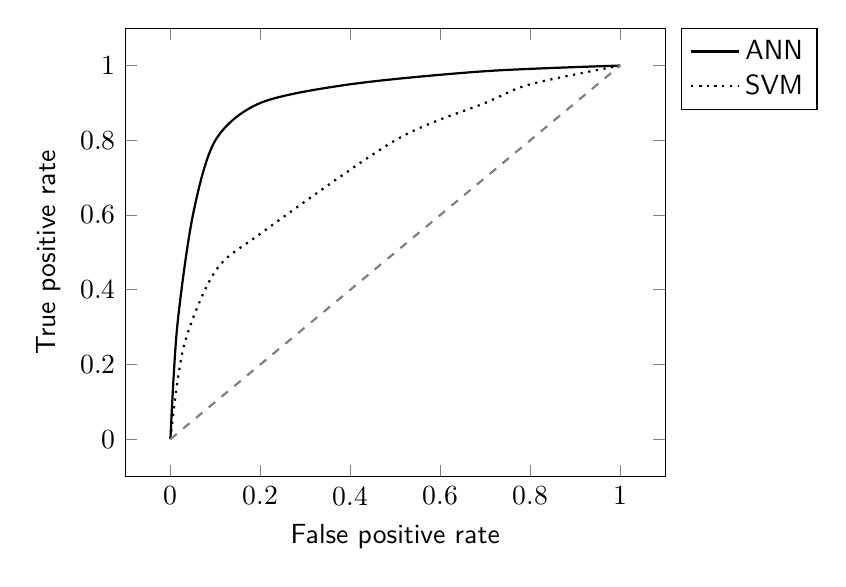
\begin{tikzpicture}
    \begin{axis}[%
      legend pos=outer north east,
      xlabel={False positive rate},
      ylabel={True positive rate}]

      \addplot[smooth, thick] coordinates {
        (0, 0) (0.015, 0.3) (0.05, 0.6) (0.1, 0.8) (0.2, 0.9) (0.4, 0.95) (0.7, 0.985) (1, 1)};
      \addlegendentry{ANN}

      \addplot[smooth, thick, dotted] coordinates {
        (0, 0) (0.03, 0.25) (0.1, 0.45) (0.2, 0.55) (0.5, 0.8) (0.7, 0.9) (0.8, 0.95) (1, 1)};
      \addlegendentry{SVM}

      \addplot[color=gray, thick, dashed] coordinates {
        (0, 0) (1, 1)};
    \end{axis}
  \end{tikzpicture}

\end{document}
